%% This is file `elsarticle-template-1-num.tex',
%%
%% Copyright 2009 Elsevier Ltd
%%
%% This file is part of the 'Elsarticle Bundle'.
%% ---------------------------------------------
%%
%% It may be distributed under the conditions of the LaTeX Project Public
%% License, either version 1.2 of this license or (at your option) any
%% later version.  The latest version of this license is in
%%    http://www.latex-project.org/lppl.txt
%% and version 1.2 or later is part of all distributions of LaTeX
%% version 1999/12/01 or later.
%%
%% Template article for Elsevier's document class `elsarticle'
%% with numbered style bibliographic references
%%
%% $Id: elsarticle-template-1-num.tex 149 2009-10-08 05:01:15Z rishi $
%% $URL: http://lenova.river-valley.com/svn/elsbst/trunk/elsarticle-template-1-num.tex $
%%
%\documentclass[preprint,12pt]{article}
\documentclass[11pt,oneside,a4paper]{article}


%% Use the option review to obtain double line spacing
%% \documentclass[preprint,review,12pt]{elsarticle}

%% Use the options 1p,twocolumn; 3p; 3p,twocolumn; 5p; or 5p,twocolumn
%% for a journal layout:
%% \documentclass[final,1p,times]{elsarticle}
%% \documentclass[final,1p,times,twocolumn]{elsarticle}
%% \documentclass[final,3p,times]{elsarticle}
%% \documentclass[final,3p,times,twocolumn]{elsarticle}
%% \documentclass[final,5p,times]{elsarticle}
%% \documentclass[final,5p,times,twocolumn]{elsarticle}

%% The graphicx package provides the includegraphics command.
\usepackage{graphicx}
%% The amssymb package provides various useful mathematical symbols
\usepackage{amssymb}
\usepackage{cite}
\usepackage{floatrow}
\newfloatcommand{capbtabbox}{table}[][\FBwidth]
\usepackage{capt-of}% or \usepackage{caption}
%% The amsthm package provides extended theorem environments
%% \usepackage{amsthm}
\usepackage{tabularx}
%% The lineno packages adds line numbers. Start line numbering with
%% \begin{linenumbers}, end it with \end{linenumbers}. Or switch it on
%% for the whole article with \linenumbers after \end{frontmatter}.
\usepackage{lineno}
\usepackage{multicol}
\usepackage[letterpaper, margin=1.4in]{geometry}
\usepackage{hyperref}
\usepackage{enumitem}
\setlist{leftmargin=4.5mm}

\usepackage{lipsum}
\newenvironment{Figure}
{\par\medskip\noindent\minipage{\linewidth}}
{\endminipage\par\medskip}
%% natbib.sty is loaded by default. However, natbib options can be
%% provided with \biboptions{...} command. Following options are
%% valid:

%%   round  -  round parentheses are used (default)
%%   square -  square brackets are used   [option]
%%   curly  -  curly braces are used      {option}
%%   angle  -  angle brackets are used    <option>
%%   semicolon  -  multiple citations separated by semi-colon
%%   colon  - same as semicolon, an earlier confusion
%%   comma  -  separated by comma
%%   numbers-  selects numerical citations
%%   super  -  numerical citations as superscripts
%%   sort   -  sorts multiple citations according to order in ref. list
%%   sort&compress   -  like sort, but also compresses numerical citations
%%   compress - compresses without sorting
%%
%% \biboptions{comma,round}

% \biboptions{}

%\journal{Journal Name}
\date{}
\begin{document}
%\begin{frontmatter}
%% Title, authors and addresses

\title{Classify Amazon Rainforest Pattern Using Satellite Data}
\maketitle
%% use the tnoteref command within \title for footnotes;
%% use the tnotetext command for the associated footnote;
%% use the fnref command within \author or \address for footnotes;
%% use the fntext command for the associated footnote;
%% use the corref command within \author for corresponding author footnotes;
%% use the cortext command for the associated footnote;
%% use the ead command for the email address,
%% and the form \ead[url] for the home page:
%%
%% \title{Title\tnoteref{label1}}
%% \tnotetext[label1]{}
%% \author{Name\corref{cor1}\fnref{label2}}
%% \ead{email address}
%% \ead[url]{home page}
%% \fntext[label2]{}
%% \cortext[cor1]{}
%% \address{Address\fnref{label3}}
%% \fntext[label3]{}


%% use optional labels to link authors explicitly to addresses:
%% \author[label1,label2]{<author name>}
%% \address[label1]{<address>}
%% \address[label2]{<address>}

\author{Yao Weng}

%\address{California, United States}

\begin{abstract}
%% Text of abstract
In recent decades, scientists have studied the deforestation patterns using satellite data, and indicate that Amazon rainforest deforestation is rapidly accelerating. Kaggle together with Planet, designer and builder of the world’s largest constellation of Earth-imaging satellites, hold a competition to apply satellite data to track the human footprint in the Amazon rainforest. The labeled satellite image chips are provided by Planet and its Brazilian partner SCCON (Santiago $\&$ Cintra Consultoria), I will develop an algorithm to classify the image using what I have learned in Machine Learning Engineer Nanodegree Program.
\end{abstract}

%\begin{keyword}
%Science \sep Publication \sep Complicated
%% keywords here, in the form: keyword \sep keyword

%% MSC codes here, in the form: \MSC code \sep code
%% or \MSC[2008] code \sep code (2000 is the default)

%\end{keyword}

%\end{frontmatter}

%%
%% Start line numbering here if you want
%%
%\linenumbers
\begin{multicols}{2}
%% main text
\section{Domain Background}
\label{S:1}
Satellites are very powerful tools to detect deforestation of rainforest.The National Institute for Space Research (INPE) have developed a near real-time deforestation detection system (DETER) and it has helped Brazil’s government to reduce its deforestation rate by almost $80\%$ since 2004\cite{amazonnature}. In April 21th 2017, Kaggle launched a competition of Understanding the Amazon from Space. It encourages competitors to apply machine learning algorithms to label satellite image chips with atmospheric conditions and various classes of land cover/land use \cite{amazonkaggle}. I choose this topic as my capstone project for two major reasons. First, it is worthy to develop an algorithm to precisely classify the rainforest satellite images, as it will help scientists to do offline study of the deforestation pattern, rate and then better understanding the problem. Secondly, a fast algorithm can be applied in the real-time system which can help scientists or governments to quickly respond to the on-going deforestation.

\section{Problem Statement}
\label{S:2}
The chips (image) were derived from Planet's full-frame analytic scene products using our 4-band satellites in sun-synchronous orbit and International Space Station orbit. They were labeled using the Crowd Flower platform and a mixture of crowd-sourced labor and Berlin and San Francisco teams of Planet, the whole processing is time consuming and costly.

The labels can broadly be broken into three groups: a) atmospheric conditions, b) common land cover/land use phenomena, and c) rare land cover/land use phenomena. An image may have one and potentially more than one atmospheric label, and zero or more common and rare labels, shown in Fig.\ref{fig:sample}. The task is to assign a chip a set of target labels, which can be considered as a multi-label classification.

\begin{Figure}
 \centering
 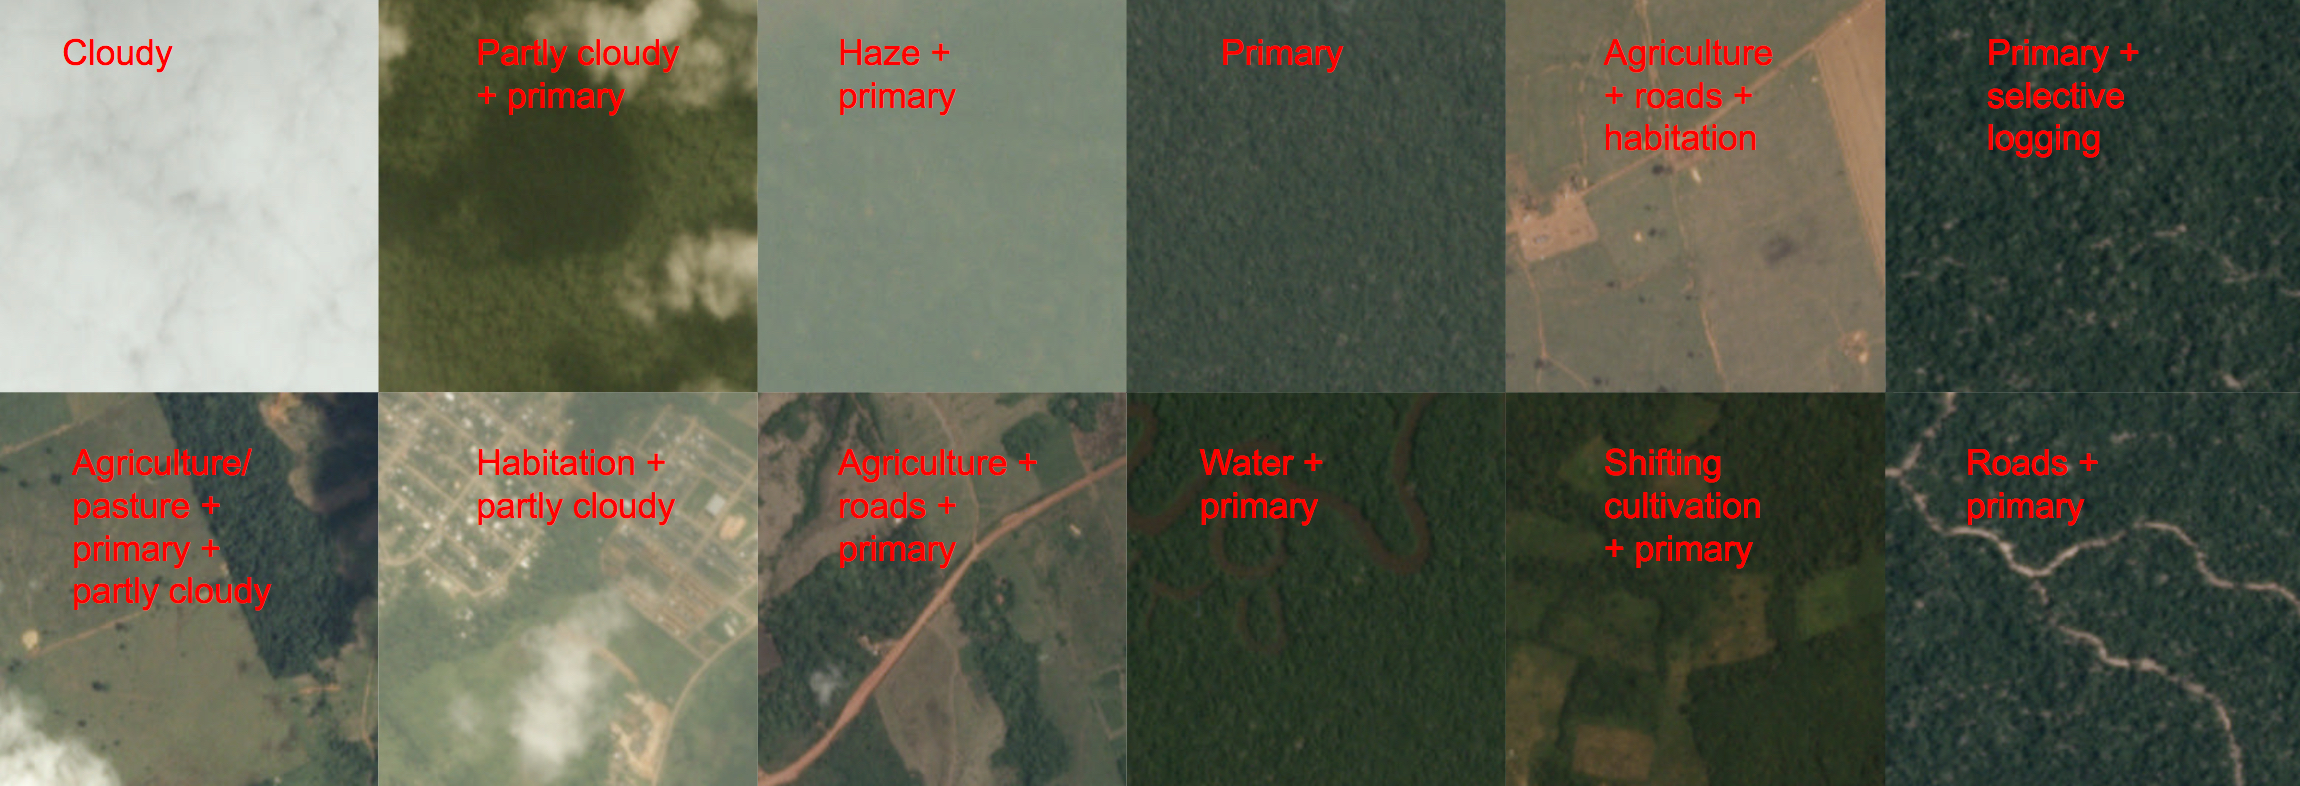
\includegraphics[width=\linewidth, height=0.4\linewidth]{chips.jpg}
 \captionof{figure}{Sample chips and their labels.}\label{fig:sample}
\end{Figure}

\section{Datasets and Input}
\label{S:3}
Data\cite{amazonkaggle} are composed of 40479 labeled training images and 61191 unlabeled images for final submission. The file size of an image is ${256\times 256 \times 3}$, Tab.\ref{tab:labels} shows the label distributions of the training data.

\small{
\begin{Figure}
\begin{tabularx}{1\columnwidth}{l|l|l}
\hline
\hline
Atmospheric & cloudy & 2089 \\ 
  & partly cloundy &  7261 \\  
  & haze &   2697 \\
  & clear &   28431 \\
\hline 
Common Land & primary & 37513 \\
 & water & 7411 \\
 & habitation & 3660 \\
 & agriculture & 12315 \\
 & road & 8071 \\
 & cultivation & 4477 \\
 & bare ground & 862 \\
\hline
Rare Land & slash burn & 209 \\
 & selective logging & 340 \\
 & blooming & 332 \\
 & conventional mine & 100 \\
 & artisinal mine & 339 \\
 & blow down & 98 \\ \hline
\end{tabularx}
\captionof{table}{Label classification of training data.}\label{tab:labels}
\end{Figure}
}


%\begin{figure}[h]
%\centering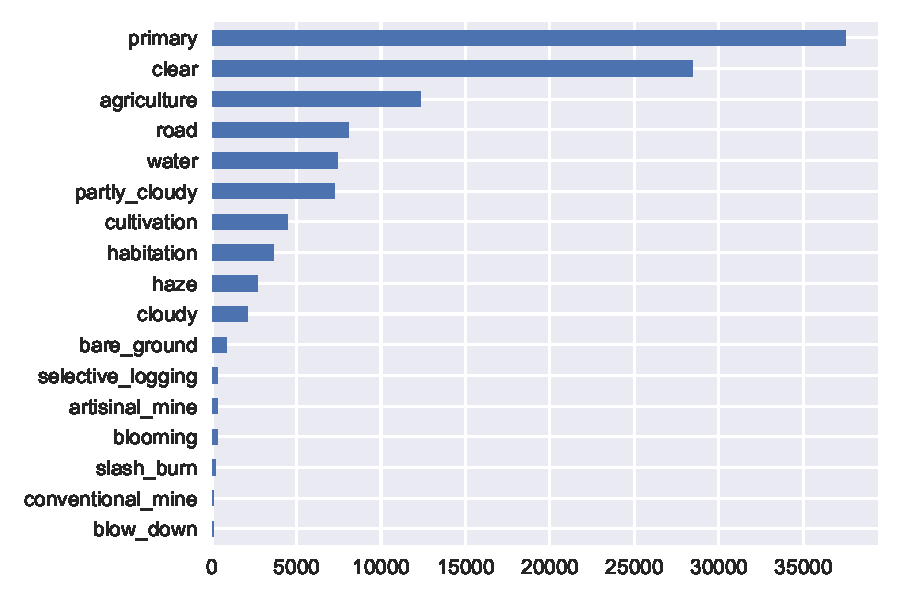
\includegraphics[width=0.6\linewidth]{amazon_labels.pdf}
%\caption{Label frequencies of training data.}
%\end{figure}  

%blow_down               98
%conventional_mine      100
%slash_burn             209
%blooming               332
%artisinal_mine         339
%selective_logging      340
%bare_ground            862
%cloudy                2089
%haze                  2697
%habitation            3660
%cultivation           4477
%partly_cloudy         7261
%water                 7411
%road                  8071
%agriculture          12315
%clear                28431
%primary              37513
  
\section{Solution and Statement}
\label{S:4}
There are two main methods to solve multi-label classification problem. One is to transform the multi-label problem into single-abel problems(s), but the transformed dataset grows large with high label cardinality and cannot model dependencies between labels. The other one is to adapt a single-label algorithm to produce multi-label outputs. In this competition, I will adapt conventional neural network with multiple outputs.

\subsection{Loss Function}
In single label classification, we use softmax function to squash the values of a vector in the range $[0,1]$ that add up to 1. In multi-label case, a sigmoid function Eq.\ref{eq:sigmoid} is used to predict the outputs, which indicates the class probabilities. I set $0.5$ to the threshold of tagging a class, if the predicated class probability is greater than this threshold, the image is labeled with this class.

\begin{equation}
\sigma(x) = \frac{1}{1 + \exp{(-x)}} \label{eq:sigmoid}
\end{equation}

Binary cross entropy function is used as loss function Eq.\ref{eq:loss},
\begin{eqnarray}
\mathcal{L}(\theta) & = &  
-\frac{1}{n}\sum^{n}_{i=1}\left[y_i \log(p_i) + (1-y_i)\log(1-p_i)\right] \nonumber \\
& = & -\frac{1}{n}\sum^{n}_{i=1}\sum^{m}_{j=1}y_{ij}\log(p_{ij}) \label{eq:loss}
\end{eqnarray}
where $i$ sums over all samples and $j$ sums over all classes, $y$ is the sample label and $p_{ij}\in(0,1)$,$\sum_{j} p_{ij} = 1 \forall i, j$ is the prediction for a sample.

\subsection{Measurement Metrics}
The $F_2$ score is used to evaluate the submission, see Eq.\ref{eq:f2}
\begin{equation}
F_{2} = (1+\beta^{2})\frac{pr}{\beta^2 p + r}, \beta = 2 \label{eq:f2}
\end{equation}
where Precision $p$ is the ratio of true positives to all predicted positives. Recall $r$ is the ratio of true positives to all actual positives. $F_2$ weights recall higher than precision, the mean $F_2$ score is formed by averaging the individual $F_2$ scores for each row in the test data. 

\subsection{Baseline Model}
Convolutional neural network (CNN) has demonstrated excellent performance on many complex visual tasks. My baseline model is a two layer CNN with three fully connected  layers. Each fully connected layer is followed by a pooling layers with drop probability $0.3$. Fig.\ref{fig:cnngraph} shows the architecture of baseline CNN. Training data is splitted to training set ($80\%$) and testing set ($20\%$), the image is resize to $128\times 128\times 3$. Data is trained in $50$ epochs with batch size of $128$. I submitted the predictions using baseline model, the $F_2$ score is $0.82681$. The best $F_2$ score in the competition is $0.93423$, and the sample submission benchmark from Kaggle is $0.67485$. Fig.\ref{fig:train9252} shows one misclassification in common land feature, the baseline model failed to tag 'water'.

\begin{Figure}
 \centering
 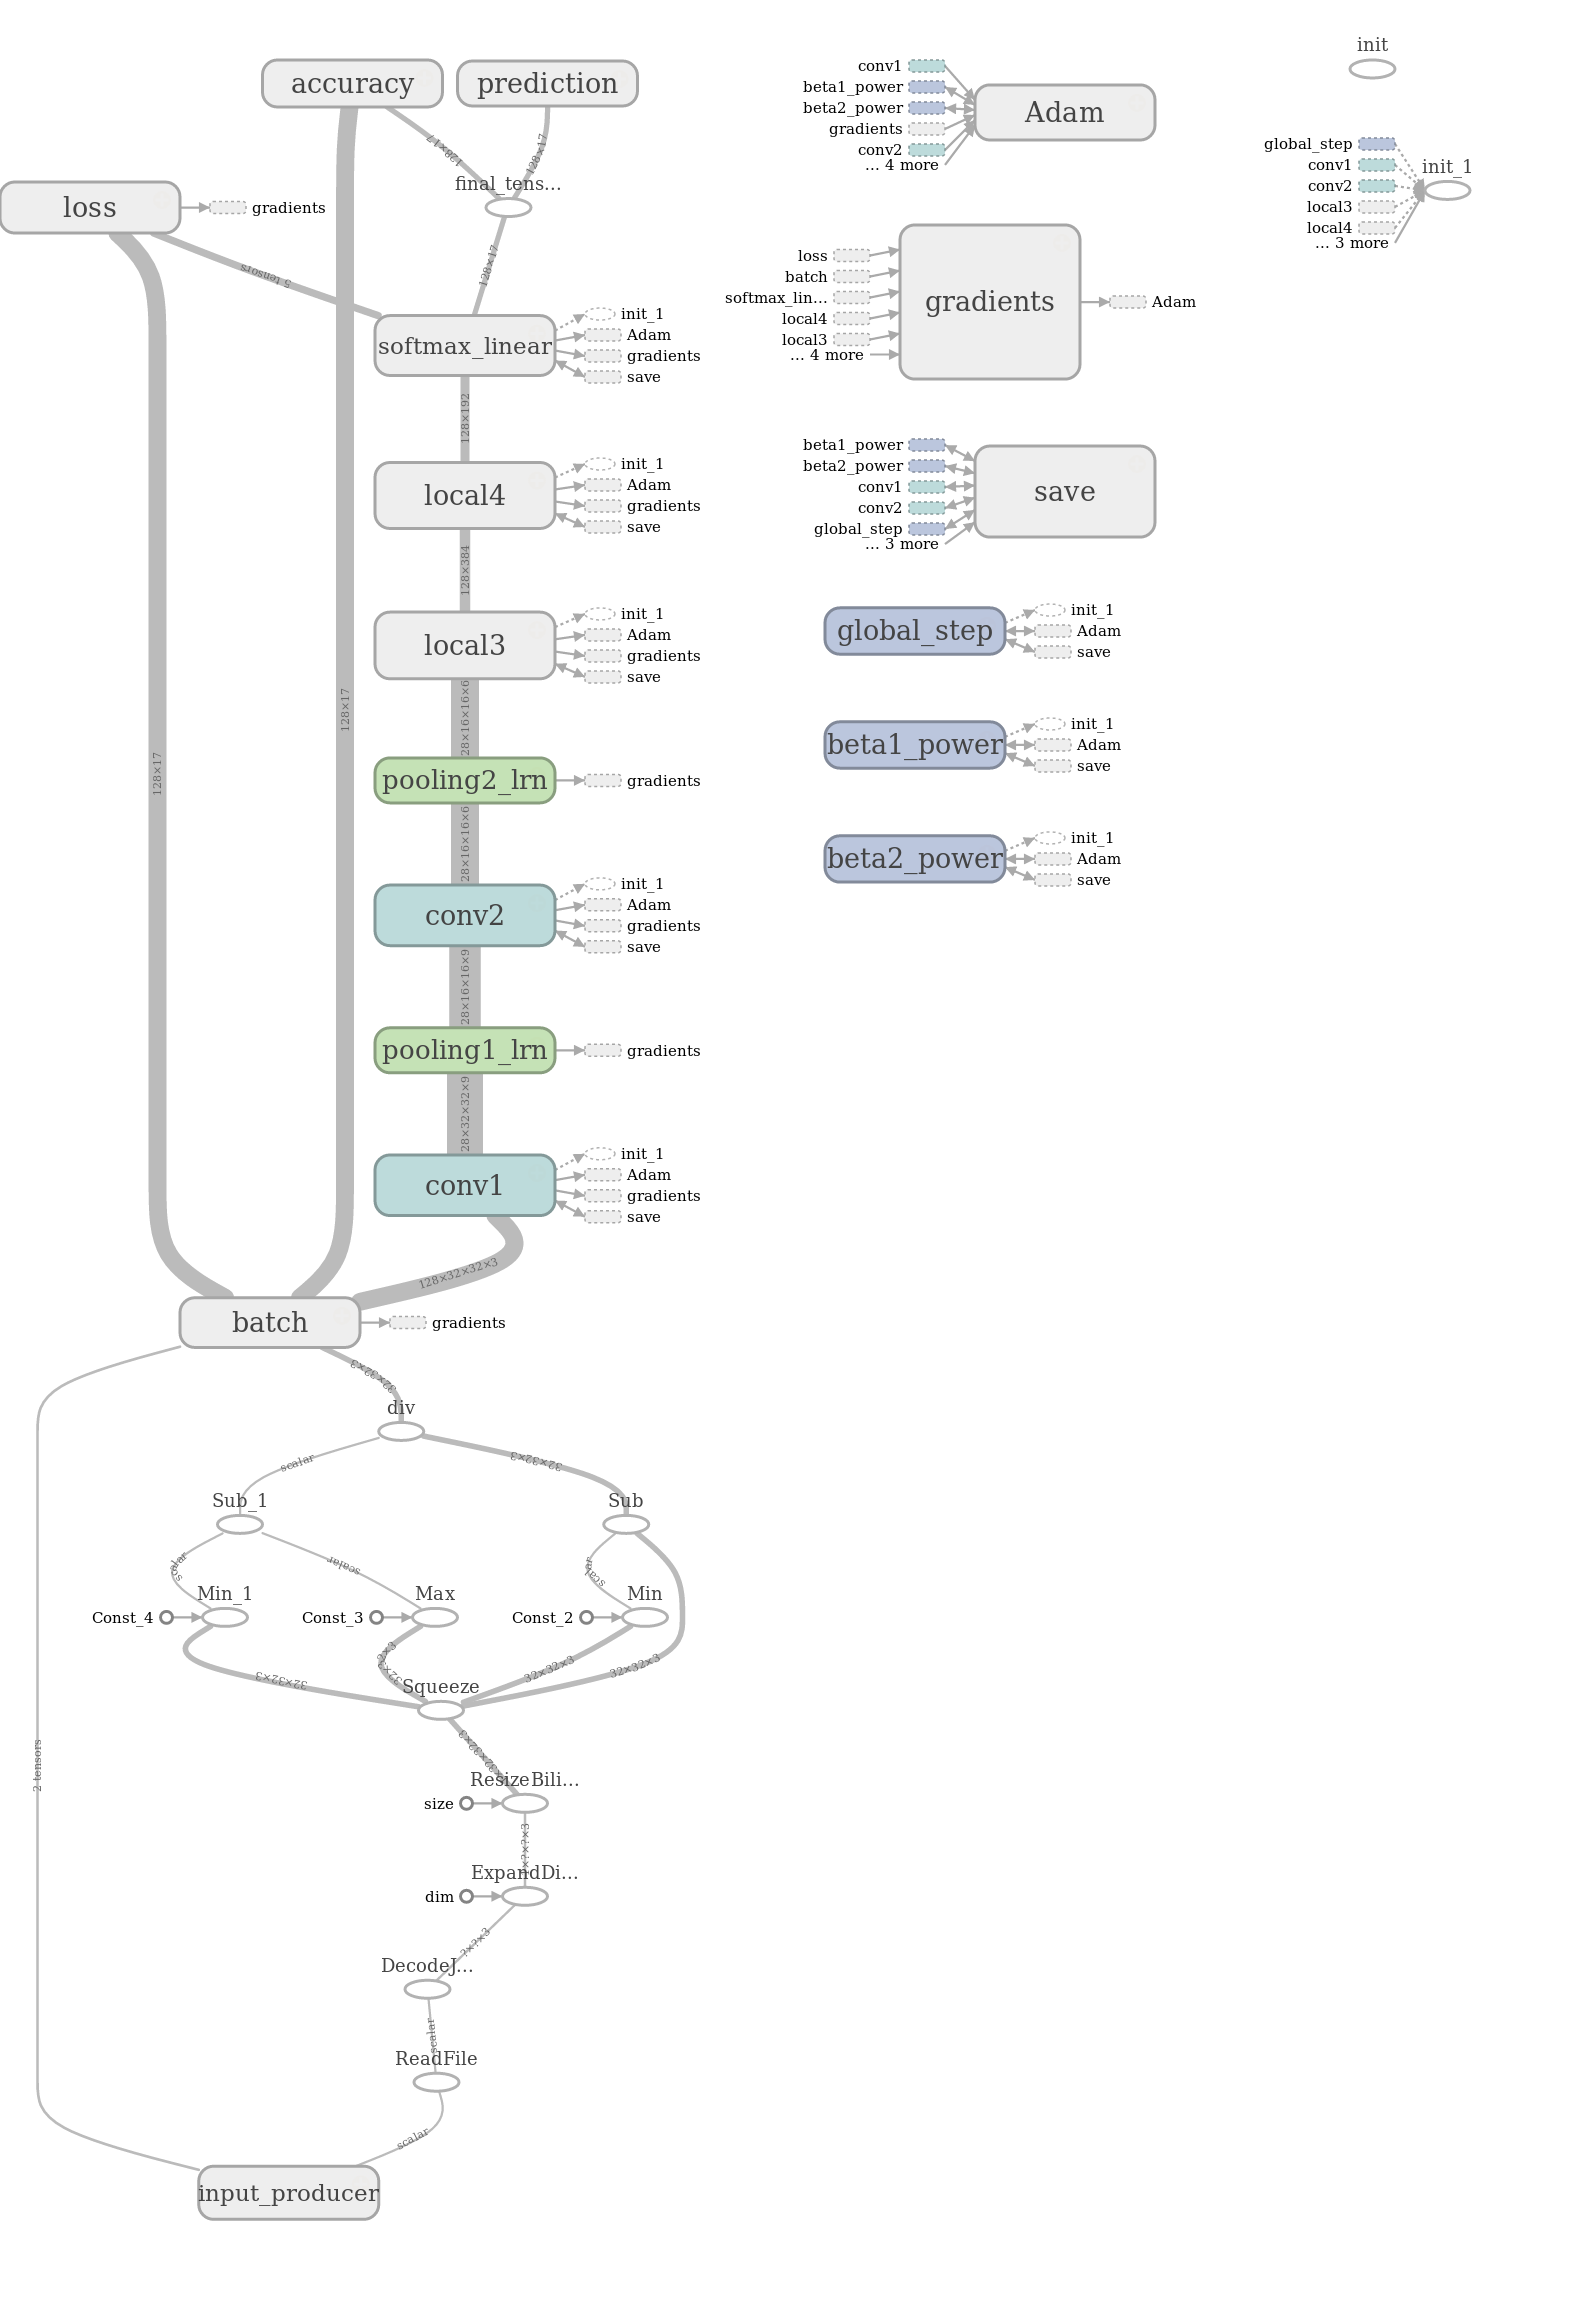
\includegraphics[width=\linewidth, height=1.5\linewidth]{baseline_graph.png}
 \captionof{figure}{Tensorboard: baseline CNN architecture.}\label{fig:cnngraph}
\end{Figure}

\begin{Figure}
 \centering
 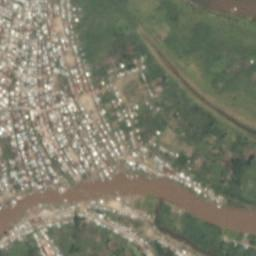
\includegraphics[width=0.6\linewidth]{train_9252.jpg}
 \captionof{figure}{True Label: agriculture clear habitation primary road water. Prediction: agriculture clear habitation primary road}\label{fig:train9252}
\end{Figure}

\subsection{Transfer Learning}
Transfer learning involves taking a pre-trained neural network and adapting the neural network to a new different data set and thus accelerate our deep learning model.There are two major methods in transfer learning: retraining and fine tuning, depending on the size of new data set and the similarity of new data to the original data. The amazon satellite image data set is not big, however, is different from ImageNet which used to train Inception v3, VGG16 etc. In this capstone project, I will apply transfer learning using Inception v3. I will modify the last fully-connected layer in shape of $1\times1\times17$, where $17$ is the total number of classes of amazon images. Freeze all the weights from the pre-trained networks except the last layer, retrain the network to update the weights of the new fully connected layer.




%% appendix sections are then done as normal sections
%% \appendix

%% \section{}
%% \label{}

%% References
%%
%% Following citation commands can be used in the body text:
%% Usage of \cite is as follows:
%%   \cite{key}          ==>>  [#]
%%   \cite[chap. 2]{key} ==>>  [#, chap. 2]
%%   \citet{key}         ==>>  Author [#]

%% References with bibTeX database:
%\bibliography{mybib}{}
\bibliographystyle{plain}{}
\bibliography{sample}

%% Authors are advised to submit their bibtex database files. They are
%% requested to list a bibtex style file in the manuscript if they do
%% not want to use model1-num-names.bst.

%% References without bibTeX database:

% \begin{thebibliography}{00}

%% \bibitem must have the following form:
%%   \bibitem{key}...
%%

% \bibitem{}

% \end{thebibliography}

\end{multicols}
\end{document}

%%
%% End of file `elsarticle-template-1-num.tex'.